% !TeX root = ../main.tex
\subsection{现有实现的补充验证}\label{minor:supplement}
以下两组对照分别检验代表日压缩与建筑热状态耦合，比较条件与结果见表\ref{tab:r8p-comparisons}。

\textbf{真实负荷的权重对照。}E01预先冻结开发集外6栋BDG2计量建筑\supcite{29}，涵盖热水、蒸汽、冷水，每栋取2017年，以同一组8--10个实际代表日比较频数、软能量校准与硬能量最小$W_1$权重。标准线性规划同时约束总日数、完整日能量与极端日权重下界，归一$W_1$中位数由软校准的12.3150\%降至4.4775\%。六例线性规划均成功，但完整统计准入仅由3/6增至4/6；两例因原观测峰被完整日筛选丢失而拒绝，回退也未达标。筛选排除了4.59\%--34.79\%的已观测能量，改善只对保留完整日成立，不能据此认定规划或运行可用。

\begin{table}[H]
\centering
\caption{两组代表性对照的完整比较口径}\label{tab:r8p-comparisons}
\begin{tabularx}{\linewidth}{@{}Yrr@{}}
\toprule
\multicolumn{3}{@{}l}{E01：同六栋建筑、同一实际日集合}\\
权重方法 & 归一$W_1$中位数/\% & 统计准入/6\\\midrule
极端日频数 & 15.4450 & 0\\
软能量校准 & 12.3150 & 3\\
硬能量最小$W_1$ & 4.4775 & 4\\
\bottomrule
\end{tabularx}
\par\vspace{4pt}
\begin{tabularx}{\linewidth}{@{}Yrrrr@{}}
\toprule
\multicolumn{5}{@{}l}{E03：双楼2880小时，热容倍率与公用电上限$2\times2$}\\
$C_B$倍率/电上限 & 电量费/元 & 电量/kWh & CO$_2$/kg & 峰值/kW\\\midrule
1/无 & 5918.14 & 8155.11 & 3297.93 & 14.1064\\
4/无 & 5490.94 & 8725.44 & 3528.57 & 25.3335\\
1/有 & 5937.64 & 8050.61 & 3255.67 & 6.4796\\
4/有 & 5660.96 & 8386.07 & 3391.33 & 6.4796\\
\bottomrule
\end{tabularx}
\end{table}

\begin{figure}[htbp]
\centering
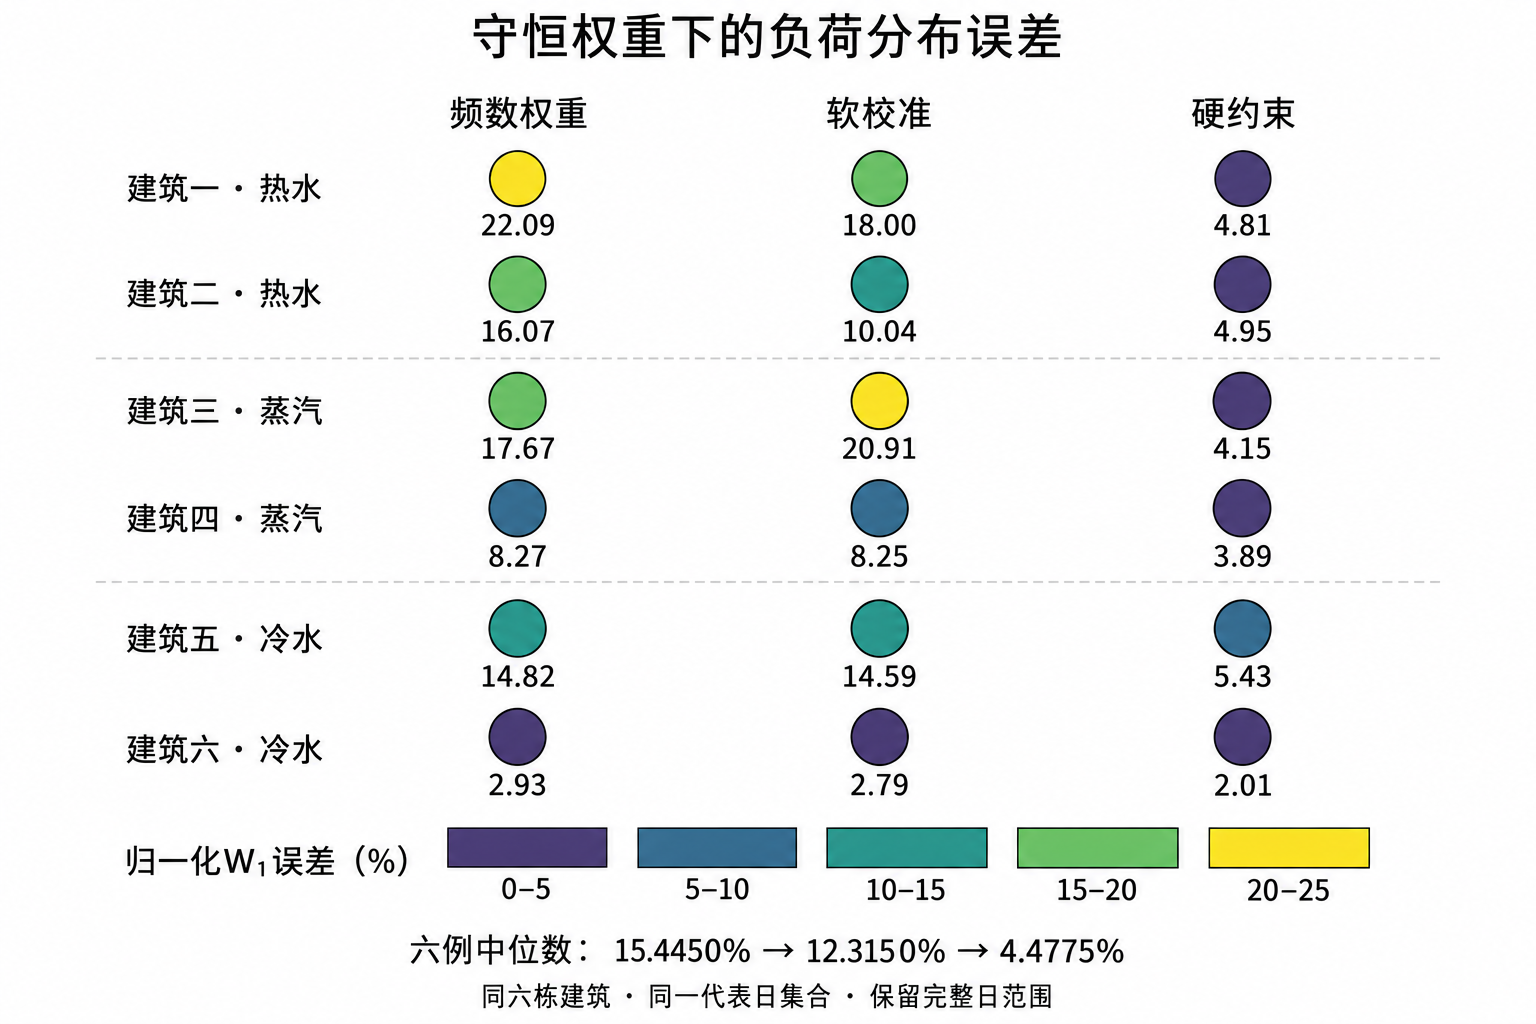
\includegraphics[width=0.93\linewidth]{results-a3/bdg2_data_a3.png}
\caption[同一代表日集合下的六楼负荷分布误差]{同一代表日集合下的六楼负荷分布误差。圆点颜色按归一$W_1$误差分箱，数值单位为\%；区间左闭右开，末档包含25。建筑一至六依次对应附录5.1的Alissa、Ian、Brandon、Genoveva、Angela、Dorethea；统计采用结果另见完整分母表。}
\label{fig:r8p-bdg2-a3}
\end{figure}

\textbf{热容与配电边界的耦合。}E03保持同一武汉公开格点天气\supcite{31}、热损系数、得热、理想设备及20--27~$^\circ$C服务，仅改变B楼热容倍率和公用电上限，连续继承2880小时状态并恢复初末20~$^\circ$C。无电上限时，四倍热容使电量费降低427.20元，却增加570.33~kWh用电；加上6.4796~kW公用上限后，省费缩为276.68元，用电仍增加335.46~kWh，费用交互为150.52元。四格求解gap均为0，独立状态、热量及配电核验通过，结论限于登记模型的固定资产运行。该对照展示用户侧热惯性向系统约束传递的可检验作用，同时区分省费、削峰与节能。其余实验、失败分母及记录路径见附录5、表\ref{tab:minor-evidence}，不与原三城工程算例的收益合并。

\begin{figure}[htbp]
\centering
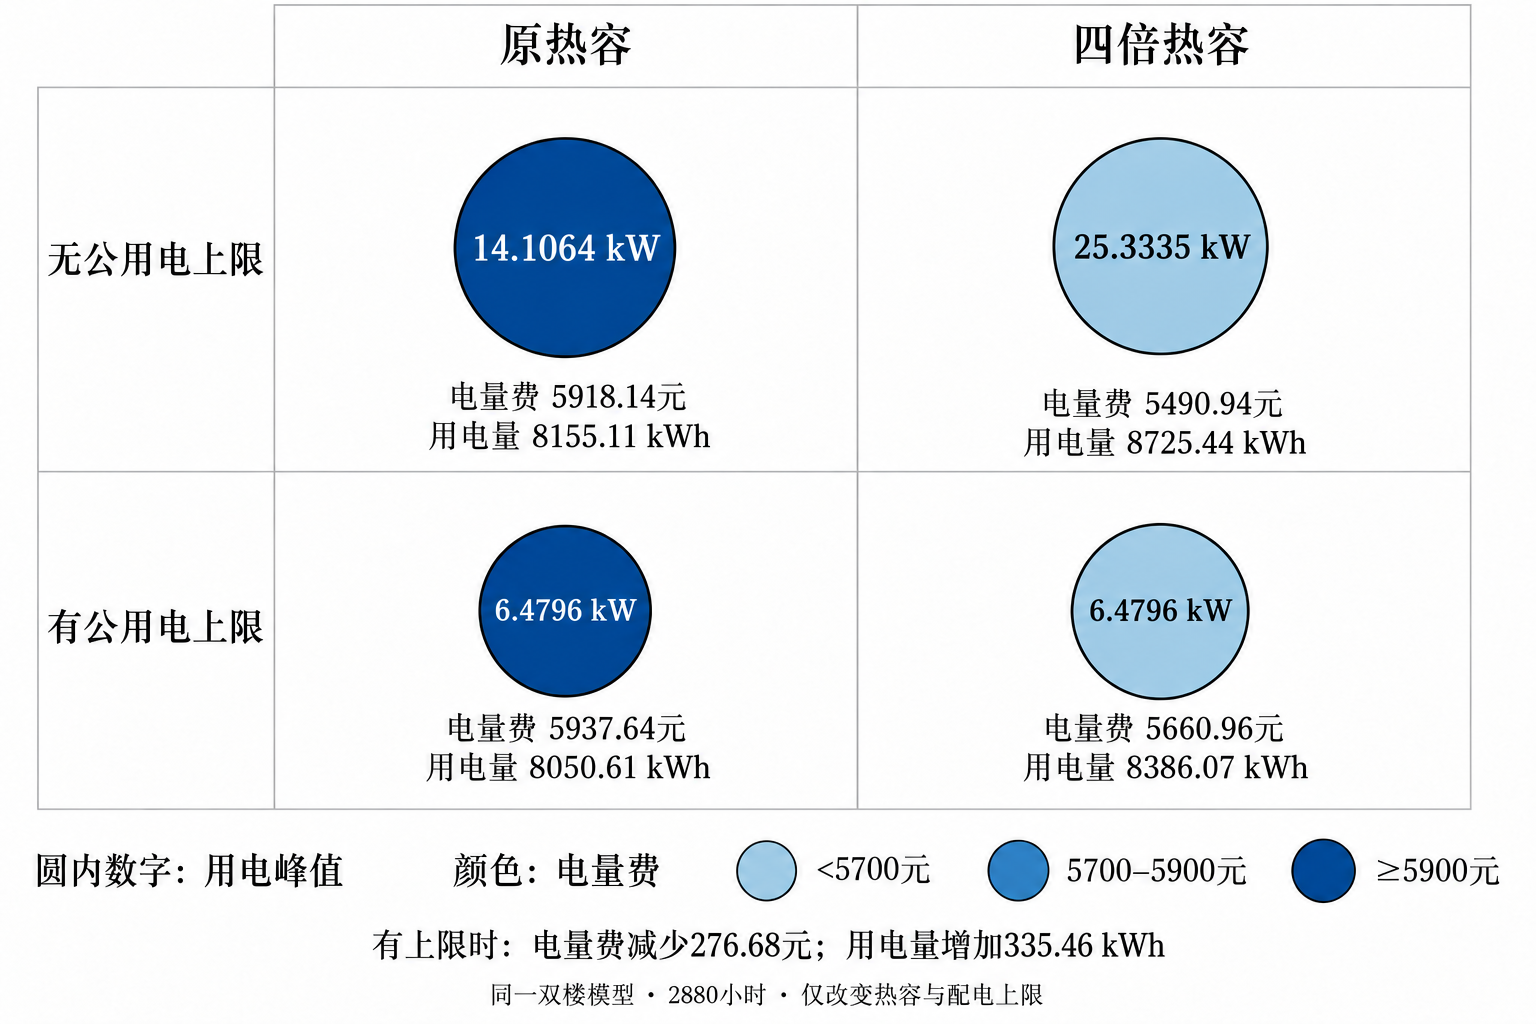
\includegraphics[width=0.95\linewidth]{results-a3/thermal_factorial_a3.png}
\caption[热容与公用电上限的四格对照]{热容与公用电上限的四格对照，仅调整B楼热容倍率。圆内标注用电峰值，颜色对应电量费区间，圆面积不作定量读数。相同配电上限下，增大热容保留移峰节费空间；电量变化与费用变化分别核算。}
\label{fig:r8p-thermal-a3}
\end{figure}
